\documentclass{article}
\usepackage[frenchb]{babel}
\usepackage{amsfonts}
\usepackage{amsmath}
\usepackage[T1]{fontenc}
\usepackage[utf8]{inputenc}
\usepackage{amsthm}
\usepackage{graphicx}
\usepackage{tikz}
\usepackage{tikz-cd}
\usepackage{hyperref}

\hypersetup{                    % parametrage des hyperliens
    colorlinks=true,                % colorise les liens
    breaklinks=true,                % permet les retours à la ligne pour les liens trop longs
    urlcolor= blue,                 % couleur des hyperliens
    linkcolor= blue,                % couleur des liens internes aux documents (index, figures, tableaux, equations,...)
    citecolor= cyan               % couleur des liens vers les references bibliographiques
    }

\title{Histoires gaussiennes }
\date{}
\author{ Clément Dell'Aiera}


\newtheorem{definition}{Definition}
\newtheorem{thm}{Théorème}
\newtheorem{ex}{Exercice}
\newtheorem{lem}{Lemme}
\newtheorem{dem}{Preuve}
\newtheorem{prop}{Proposition}
\newtheorem{cor}{Corollaire}

\newcommand{\Z}{\mathbb Z}
\newcommand{\R}{\mathbb R}
\newcommand{\C}{\mathbb C}
\newcommand{\Hil}{\mathcal H}
\newcommand{\Mn}{\mathcal M _n (\mathbb C)}
\newcommand{\K}{\mathbb K}
\newcommand{\B}{\mathbb B}
\newcommand{\Cat}{\mathbb B / \mathbb K}

\begin{document}
\maketitle

\begin{figure}[!h]\centering
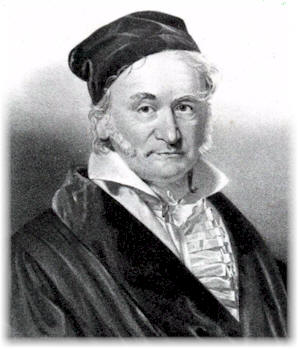
\includegraphics[scale=0.4]{Gauss2.jpg}
\caption{Gauss}
\label{fig:Gauss2}
\end{figure}

\newpage
\newpage

%\section{Problèmes antiques}
%Quadrature du cercle
%Duplication du cube
%Trisection de l'angle
%%%%%%%%%%%%%%%%%%%%%%%%%%%%%%%%%%%%%%%%%%%%%%%%%%%%%%%%%%%%%%%%%%%%%%%%%%%%%%%%%%%%%%%%%
%%%%%%%%%%%%%%%%%%%%%%%%%%%%%%%%%%%%%%%%%%%%%%%%%%%%%%%%%%%%%%%%%%%%%%%%%%%%%%%%%%%%%%%%%

%FAIRE UNE INTRO ET UNE CONCLUSION


\begin{figure}[!h]\centering
\begin{tikzpicture}[scale = 3]
\draw (0,0) -- (1,1);
\draw (0,0) -- (2,0);
\draw (1,1) -- (2,0);
\fill[gray] (0,0) -- (1,1) -- (1,0.5) -- cycle;
\draw[dashed] (1,0.5) -- (2,0);
\draw[dashed] (1,0.5) -- (0,0);
\draw[dashed] (1,0.5) -- (1,1);
\draw (0.75,0.6) node{$\mathcal A_3$};
\draw (0,0) node[left]{$A_1$} ;
\draw (2,0)  node[right]{$A_3$};
\draw (1,1)  node[above]{$A_2$};
\draw (1,0.5) node{$\times$};
\draw (1,0.5) node[right]{$M$};
\end{tikzpicture}
\caption{\textbf{Point de Lemoine.} L'aire grisée est proportionnelle à la coordonnée barycentrique de $M$ relative à $A_3$.}
\label{Lemoine}
\end{figure}

\begin{figure}[!h]\centering
\begin{tikzpicture}[scale = 3]
\draw (0,0) circle (1);
\draw (0,0) node{$\times$};
\draw (0,0) node[above left]{$C$};
\draw[->] (0,-1.3) -- (0,1.3);
\draw[->] (-1.3,0) -- (1.3,0);
\draw (0,1.3) node[above]{$\infty$};

\draw (1.3*0.866,0.5) node[below left]{$M$};
\draw[blue,->] (0.866,0.5) -- ++ (-0.5,0.866);
\draw[blue,->] (0.866,0.5) -- ++ (0,1);
\draw[blue] (0,0) -- ++ (2*0.866,2*0.5) ;

\draw[red,->] (0.25,0) arc (0:30:0.25);
\draw[red,->] (0.866,0.5+0.25) arc (90:120:0.25);

\end{tikzpicture}
\caption{\textbf{Latitude.} La latitude peut se mesurer en visant l'angle que fait l'étoile polaire avec l'horizon. }
\label{Latitude}
\end{figure}

\begin{figure}[!h]\centering
\begin{tikzpicture}[scale = 3]
\draw (0,0) ellipse (1.3 and 1);
\draw (0,0) node{$\times$};
\draw (0,0) node[above left]{$C$};
\draw[->] (0,-1.3) -- (0,1.3);
\draw[->] (-1.5,0) -- (1.5,0);

\draw (1.3*0.866,0.5) node[below left]{$M$};

\draw[blue,->] (1.3*0.866,0.5) -- ++ (0.5*0.866,0.5*1.3*0.5);
\draw[blue] (1.3*0.866,1.3*0.5) node[above right]{$N_\phi$};
\draw[blue,->] (1.3*0.866,0.5) -- ++ (0.5,0);
\draw[->] (1.3*0.866+0.25,0.5) arc (0:30:0.25);
\draw (1.3*0.866+0.25,0.5) node[above right]{$\phi$};

\draw[dashed] (1.3*0.866,0.5)-- ++ (0.5*1.3*0.5,-0.5*0.866);
\draw[dashed] (1.3*0.866,0.5)-- ++ (-0.5*1.3*0.5,0.5*0.866);
\draw (1.3*0.866-0.05*1.3*0.5,0.5+0.05*0.866) -- ++ (0.05*0.866,0.05*1.3*0.5) -- ++ (0.05*1.3*0.5,-0.05*0.866) ;
\end{tikzpicture}
\caption{\textbf{Forme de la Terre.} La latitude $\phi$ est donnée par l'angle entre la normale avec le plan de l'ecliptique. }
\label{Ellipse}
\end{figure}

\begin{figure}[!h]\centering
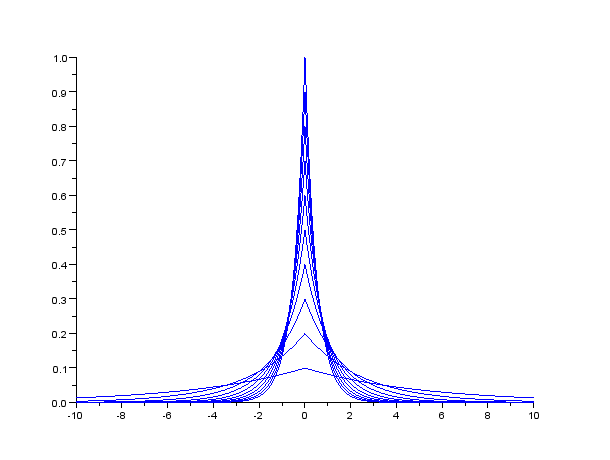
\includegraphics[scale=0.4]{Laplace.png}
\caption{Loi de l'erreur de Laplace en faisant varier le paramètre $m$ : plus il est élevé, plus l'erreur se disperse}
\label{fig:Laplace}
\end{figure}

\begin{figure}[!h]\centering
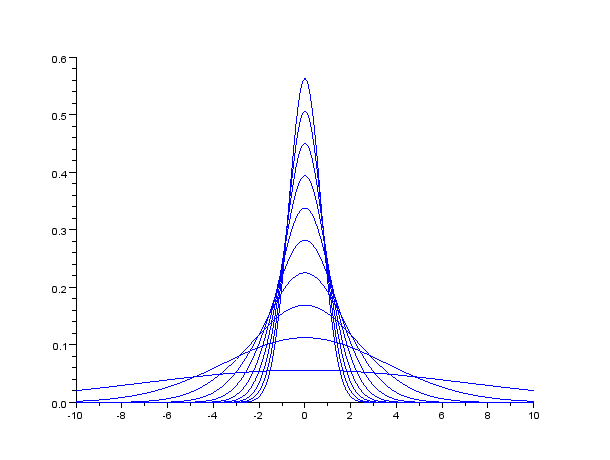
\includegraphics[scale=0.4]{Gaussienne.png}
\caption{Loi de l'erreur gaussienne en faisant varier le paramètre $h$ : plus il est élevé, plus l'erreur se disperse}
\label{fig:Gaussienne}
\end{figure}

\begin{figure}[!h]\centering
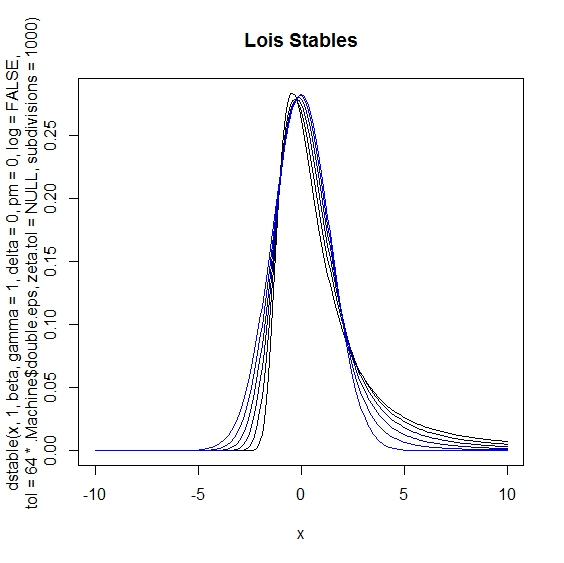
\includegraphics[scale=0.4]{Stables.jpeg}
\caption{Densité de lois stables. Plus la courbe est bleue, plus $\alpha$ se rapproche de $2$, et l'on retrouve la loi de Gauss.}
\label{fig:Stables}
\end{figure}

\end{document}


























